\chapter{La Asignación Promedio}

En este capítulo se compararán, numéricamente, las dinámicas efectivas obtenidas a través de la asignación de máxima entropía con otro tipo de asignación, con el objetivo de mostrar la dependencia fundamental de la dinámica en la aplicación de asignación y su naturaleza de estimación.

\section{Definición y acercamiento}

En el contexto de los modelos de grano grueso, otras asignaciones han sido propuestas. Nos interesamos en este capítulo en la asignación promedio \cite{Macro-To-Micro}. Esta aplicación asigna a un estado efectivo $\rho_{\ef} \in \densityspace{n}$ un estado microscópico $\varrho_{\avg} \in \densityspace{m}$ por medio de promediar sobre el conjunto de todos los estados puros microscópicos tales que son compatibles con el estado efectivo bajo una aplicación de grano grueso en particular. Dicho conjunto de estados puros microscópicos queda definido como
\begin{equation}\label{eq:Omega}
    \Omega_{\mcC}(\rho) = \{\ket{\psi}\in\hilbert_{m}:\, \mcC(\dyad{\psi}) = \rho   \}.
\end{equation}
\acnote{Una motivación física de esta asignación es que cada que se prepara un estado microscópico que sea compatible con un estado efectivo, lo que se hace es tomar un elemento del conjunto $\Omega$.}
La aplicación de asignación promedio es el promedio sobre dicho conjunto, \ie 
\begin{equation}\label{eq:AvgMap}
    \mcA_{\avg}(\rho) = \overline{\Omega_{\mcC}(\rho)} = \int d \mu\,\, \delta(\mcC(\dyad{\psi})-\rho)\,\dyad{\psi},
\end{equation}
donde $d\mu$ es la medida de Haar sobre los estados puros de $\hilbert_{m}$. La delta de Dirac asegura que únicamente se tomen en consideración a los estados puros compatibles, y la medida de Haar, que la integración sobre dicho conjunto sea uniforme. El problema de resolver (\ref{eq:AvgMap}) de forma analítica no es para nada sencillo, y es dependiente del modelo de grano grueso en cuestión. Por esta razón, en este trabajo se abordará a la aplicación de asignación promedio numéricamente.

Para hallar la asignación de un estado efectivo se generan estados puros en $\hilbert_{m}$ de manera uniforme. Todos aquellos estados cuyas imágenes bajo la aplicación de grano grueso se hallen a una distancia menor a $\epsilon$ del estado efectivo son incluidos en el cálculo del promedio. El mapeo de asignación promedio numérico queda entonces definido según
\begin{equation}\label{eq:AvgMapNum}
    \mcA'_{\avg}(\rho) = \overline{\Omega'_{\mcC}(\rho)} = \frac{1}{N}\sum_{i=1}^{N}\dyad{\psi},
\end{equation}
donde
\begin{equation}\label{eq:OmegaNum}
    \Omega'_{\mcC}(\rho) = \{\ket{\psi}\in\hilbert_{m}:\, \text{d}(\mcC(\dyad{\psi}),\rho)<\epsilon  \}.
\end{equation}
Al estado $\varrho_{\avg}$ obtenido a través de la aplicación promedio le llamaremos estado promedio.

Si el estado efectivo inicial está asociado a un sistema microscópico de $n$ qubits, es necesario generar estados de forma aleatoria y uniforme en el espacio $\hilbert_{2^{n}}$ para poder realizar el promedio. Los estados tienen dimensión $2^{n}$, y el estado promedio está caracterizado por un total de $2^{n^{2}-1}$ parámetros. Generar miles de estados de esta dimensión es computacionalmente intensivo, y en razón de esto, en este trabajo se compararán el estado promedio y el estado de máxima entropía para el caso $n=2$.

\section{Diferencia entre el MaxEnt y el AssMap}


No tenemos ninguna razón para asegurar que el estado de máxima entropía y el estado asignado por promedio son el mismo. En la asignación promedio se hacen dos suposiciones fuertes: primero, que el sistema microscópico se halla en un estado puro (aunque no asigne un estado puro al estado efectivo). Segundo, que todos los estados puros son igualmente probables. Aunque estas suposiciones puedan parecer razonables, Jaynes, en su artículo, argumenta que estas no son tan arbitrarias como cualquier otra suposición, a menos que algún tipo de simetría del sistema sugiera lo contrario.

Nos preguntamos, pues, sobre la diferencia entre el estado de máxima entropía y el estado promedio. Calculamos, pues, la distancia entre estos estados como una función del parámetro $p_{1}$ de la aplicación de grano grueso (recuérdese que en el caso $n=1$ el segundo parámetro es simplemente $1-p_{1}$). Esto es, nos interesa obtener
\begin{equation}
    \text{d}\qty(\avgass(\rho_{\ef}),\maxass(\rho_{\ef}))=\text{d}\qty(\avgass(\rho_{\ef}),\maxass(\rho_{\ef}))(p_{1}),\nonumber
\end{equation}

\begin{figure}[ht!]
    \centering
      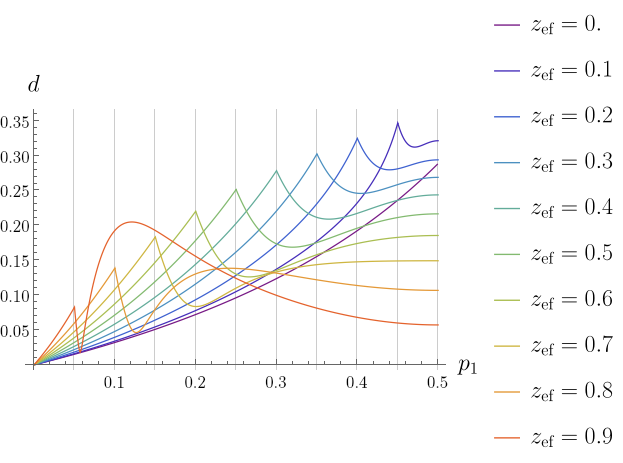
\includegraphics[width=0.9\linewidth]{chapter4/figures/maxavgdisr.png}
    \caption{Distancia entre asignaciones}
    \label{fig:AvgMaxDist}
\end{figure}

La figura  muestra que la fidelidad entre ambos estados parece constante siempre que $n>1000$, y que la verdadera dependencia se halla sobre el parámetro $p$. Veamos, pues, la fidelidad entre ambos estados como función de $p$, con $n=1000$.

La figura \ref{fig:AvgMaxDist} muestra que la distancia entre ambos estados para diferentes valores de $p_{1}$ y para diferentes valores de $r_{\ef}$. Como es natural, las asignaciones son la misma cuando el estado efectivo inicial es puro. En efecto, es sencillo demostrar que el único estado compatible con un estado efectivo inicial puro es $\rho_{\ef}^{\otimes n}$. Se ve, además, que las asignaciones coinciden también en el caso límite $p_{1}=1$ (y $p_{1}=0$ que es un caso límite únicamente cuando $n=2$).

\section{Algunas dinámicas}

\subsection{Dinámicas factorizables}

\subsection{La compuerta SWAP}

\subsection{Canales de Pauli}

\section{Comparación de resultados de ambas asignaciones}
\newpage